%-------------------------------------------------------------------------------
%                            BAB III
%               		METODOLOGI PENELITIAN
%-------------------------------------------------------------------------------

\chapter{METODOLOGI PENELITIAN}

\section{Tempat dan Waktu Penelitian}
\setlength\parindent{30pt} Penelitian ini dilakukan di Jurusan Informatika, Fakultas Matematika dan Ilmu Pengetahuan Alam, Universitas Syiah Kuala Banda Aceh. Waktu yang diperlukan untuk melakukan penelitian ini kurang lebih selama lima bulan, yang dimulai dari bulan Maret 2018 sampai bulan Juni 2018.

% Please remember to add \use{multirow} to your document preamble in order to suppor multirow cells
\begin{table}[H]
	\center
	\caption{Jadwal Penelitian.}
	\label{jadwal}
	\begin{tabular}{|c|l|l|l|l|l|l|l|}
		\hline
		\multirow{2}{*}{No} & \multirow{2}{*}{Keterangan} 	& \multicolumn{6}{c|}{Bulan}           																						\\ \cline{3-8} 
							&                           	& Maret 			& April  			& Mei 				& Juni 				& Juli 				& Agustus 				\\ \hline       
		1                   & Studi literatur           	&\cellcolor{gray}	&\cellcolor{gray}	&                   &                   &                   &                         \\ \hline
		2                   & Penulisan Proposal           	&                   &\cellcolor{gray}	&\cellcolor{gray}	&                   &                   &                         \\ \hline
		3                   & Pengembangan Aplikasi         &                   &                   & \cellcolor{gray}  & \cellcolor{gray} 	& \cellcolor{gray}  &                         \\ \hline
		4                   & Evaluasi Sistem               &                   &                   &           		&             		&\cellcolor{gray}	&   \cellcolor{gray}      \\ \hline
		5                   & Penulisan Laporan Akhir       &                   &                   &                   &        			&      				& \cellcolor{gray}        \\ \hline
	\end{tabular}
\end{table}

\section{Alat dan Bahan}
Alat yang digunakan pada penelitian ini adalah sebagai berikut :

\begin{enumerate}[a.]
\item Perangkat Keras (\textit{Hardware})
	\begin{itemize}
		\item 1 unit Laptop HP Intel(R) Core(TM) i3
		\item RAM 8 GB DDR3
		\item Harddisk 1 TB
		\item 1 unit Android Samsung S7
	\end{itemize}

\item Perangkat Lunak (\textit{Software})
	\begin{itemize}
		\item Visual Studio Code
		\item Cordova 7.0.0
		\item Ionic Framework 3
		\item SDK Android 27.0.1
	\end{itemize}
\end{enumerate}

\section{Metode Penelitian}
Skema dari alur tahapan penelitian dapat dilihat pada Gambar \ref{alur}
\vspace{-0.4cm}
\begin{figure}[H]
	\center
	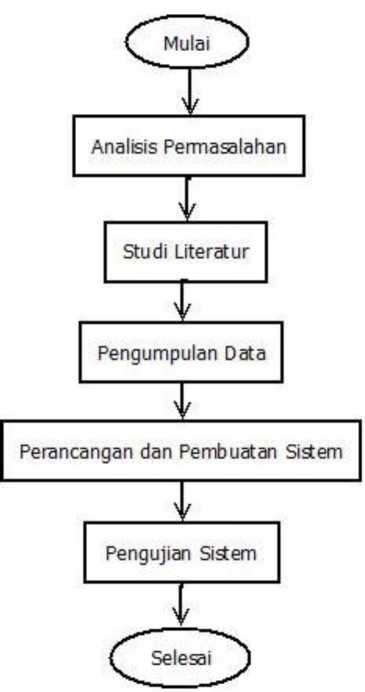
\includegraphics [width = 6cm, height= 10cm]{gambar/alur2}
	\caption{Diagram Alir Penelitian}
	\label{alur}
\end{figure}

\subsection{Analisis Permasalahan}
Aplikasi ini merupakan aplikasi berbasis mobile yang berguna untuk membantu pangkalan gas LPG Subsidi 3 Kg dalam melakukan pelaporan penyaluran tabung gas subsidi. Aplikasi ini juga membantu agen gas LPG selaku distributor dan pengawasan dari pangkalan gas untuk melakukan rekap laporan penyaluran tabung gas 3 Kg. Aplikasi ini melakukan pelaporan penyaluran tabung gas subsidi dengan cara memindai QR code yang ada pada kartu kendali milik konsumen yang di cetak sebelumnya. Setelah itu data tersebut langsung di kirim langsung ke agen gas LPG bersangkutan. Adapun fitur-fitur yang terdapat pada aplikasi ini adalah :
\begin{enumerate}[a.]
		%	\itemsep0em
		\item Masuk ke dalam aplikasi
		\item Melihat jadwal pasokan tabung 
		\item Mencatat penjualan tabung gas menggunakan NIK sebagai acuan.
		\item Mencetak kartu kendali untuk konsumen
		\item Mengubah profile biodata user
\end{enumerate}

\subsection{Studi Literatur}
Studi literatur dilakukan dengan mencari jurnal baik nasional maupun internasional, buku, serta beberapa literatur elektronik yang diunduh dari internet yang terkait dengan penelitian ini. Studi literatur juga diperoleh dari penelitian sebelumnya yang berkaitan dengan penelitian. Studi literatur digunakan sebagai bahan referensi selama proses penelitian.

\subsection{Pengumpulan Data}
Data yang digunakan dalam penelitian ini adalah data penyaluran tabung dan format pelaporan yang dipakai. Data tersebut didapatkan dari agen dan pangkalan yang menjadi objek penelitian.

\subsection{Perancangan dan Pembuatan Sistem}
Dalam merancang aplikasi ini, digunakan metode pengembangan perangkat lunak yaitu eXtreme Programming (XP). Metode XP fleksibel terhadap perubahan-perubahan sehingga cocok digunakan pada aplikasi ini. Berikut merupakan tahapan perancangan sistem yang akan dilakukan:

\begin{enumerate}[1.]
	\item \emph {Planning}
	
	Pada tahap ini dikumpulkan kebutuhan awal user atau dalam XP dikenal dengan istilah \emph {user requirement}. Hal ini dibutuhkan agar kebutuhan \emph {output} sistem, dan fitur utama dari aplikasi yang dikembangkan terdefinisikan dengan jelas. Selanjutnya dilakukan analisa kebutuhan awal terhadap aplikasi:
	
	\begin{enumerate}[a.]
		\item \textit{User Story}
		User story adalah deskripsi singkat dan sederhana mengenai fitur atau fungsi dari software, dilihat dari sudut pandang pengguna. Berikut ini merupakan user story dari kasus penelitian ini.
		\begin{itemize}
			\item \textbf{ID: 01}
			\par Sebagai pangkalan, saya ingin mencatat penjualan tabung ke dalam laporan logbook.
			\item \textbf{ID: 02}
			\par Sebagai pangkalan, saya ingin mengetahui jadwal pasokan / penerimaan tabung gas
			\item \textbf{ID: 03}
			\par Sebagai pangkalan, saya ingin melakukan login ke dalam aplikasi
			\item \textbf{ID: 04}
			\par Sebagai pangkalan, saya ingin mendaftarkan konsumen baru.
			\item \textbf{ID: 05}
			\par Sebagai agen, saya ingin melakukan rekap laporan dari masing-masing pangkalan milik saya.
			\item \textbf{ID: 06}
			\par Sebagai agen, saya ingin menetapkan kuota tabung per bulan untuk masing-masing pangkalan.
			\item \textbf{ID: 07}
			\par Sebagai pangkalan, saya ingin mencetak kartu kendali konsumen untuk pangkalan kecil yang belum memiliki mesin cetak.
		\end{itemize}
		Penggunaan nomor unik ID pada user story dilakukan untuk memudahkan pengelolaan \textit{user story} sekaligus membedakan satu \textit{user story} dengan yang lainnya.
		
		\item Kebutuhan Fungsional
		\newline Kebutuhan fungsional, dapat dimodelkan pada use case diagram. Use case diagram adalah diagram yang memodelkan perilaku dari sistem. Di dalam use case diagram terdapat sekumpulan use case, aktor dan hubungan antara use case dan aktor. Use case diagram dapat dilihat pada \ref{usecase} di bawah ini.
		
		\vspace{-0.4cm}
		\begin{figure}[H]
			\center
			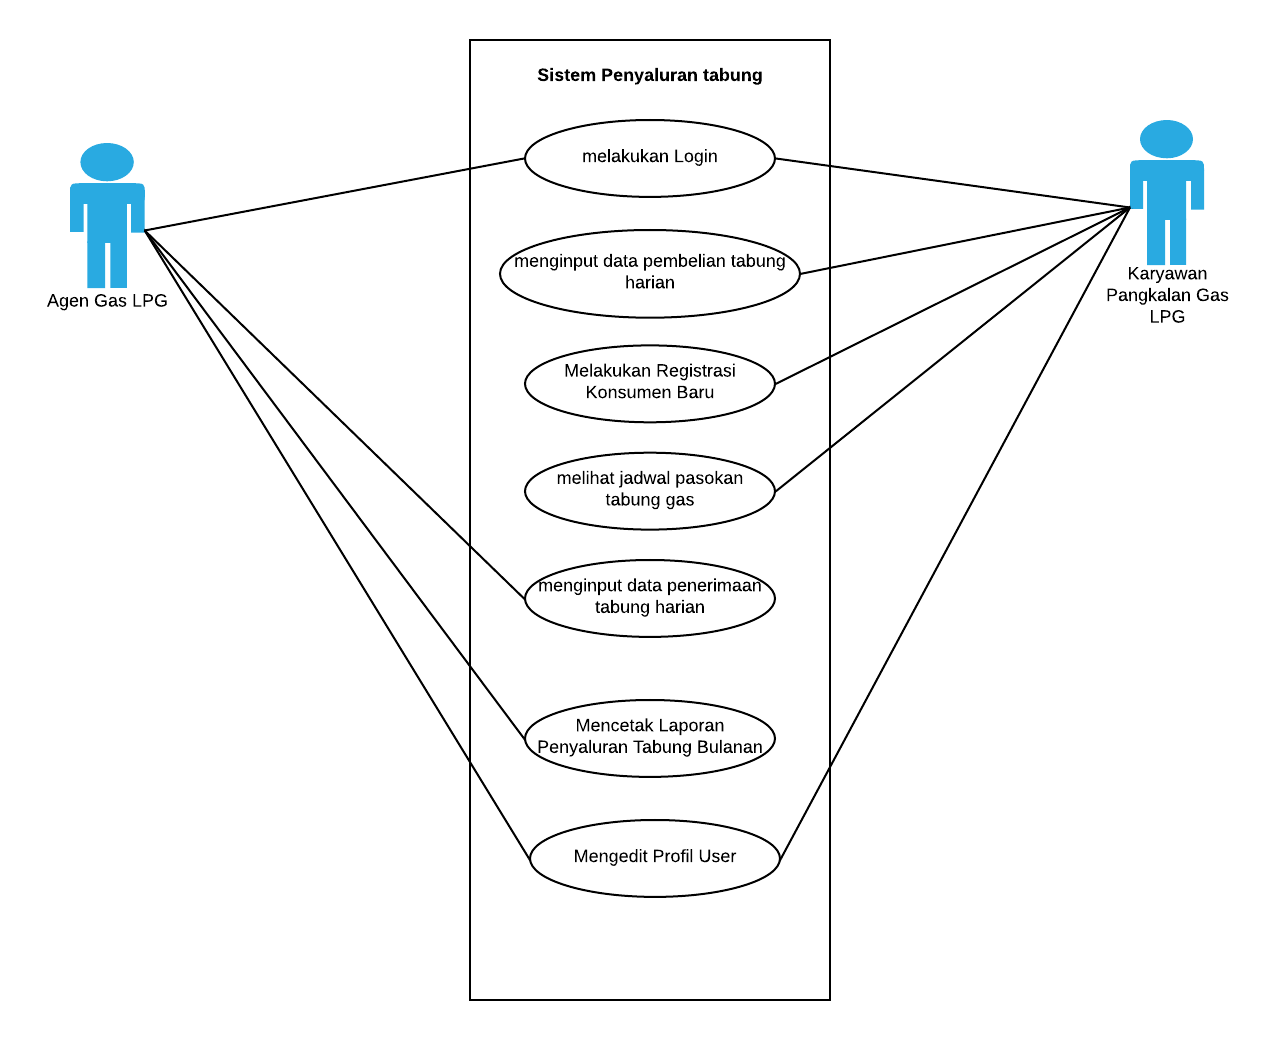
\includegraphics [width = 12cm, height= 11cm]{gambar/use-case}
			\caption{Diagram Use-Case}
			\label{usecase}
		\end{figure}
	
		\item Kebutuhan Non Fungsional
		\newline Kebutuhan non-fungsional adalah batasan dalam layanan atau fungsi yang ditawarkan sistem. Dalam penelitian ini, kebutuhan non-fungsional yang digunakan ada dua macam, seperti pada Tabel 3.2.
		
		\vspace{-0.4cm}
		\begin{table}[H]
			\centering
			\caption{Kebutuhan Non-Fungsional}
			\label{kebutuhan}
			\begin{tabular}{|l|p{5cm} |}
				\hline
				Jenis Kebutuhan & Deskripsi \\ 
				\hline 
				\textit{Usability} & Sistem yang dibuat harus dapat dipelajari dan digunakan dengan mudah oleh pengguna. Kemudahan-kemudahan tersebut diantaranya kemudahan dalam hal penggunaan sistem. \\ 
				\hline 
				\textit{Compatibility} & Sistem dapat diakses melalui beberapa versi sistem operasi Android. \\ 
				\hline 
			\end{tabular} 
		\end{table}
		
		
	\end{enumerate}

	\item \textit{Design}
	
	Tahap ini fokus pada desain pembuatan program perangkat lunak termasuk struktur data, arsitektur perangkat lunak, representasi antarmuka dan prosedur pengkodean. Representasi perangkat lunak yang dikembangkan digambarkan dalam sebuah pemodelan. Tahapan perancangan dilakukan berdasarkan dari hasil analisis kebutuhan perangkat lunak pada tahap sebelumnya. Tahapan desain ini meliputi perancangan Unified Modelling Languange (UML), perancangan database dan perancangan desain tampilan (user interface).
	
	\item \textit{Coding}
	
	Pada tahapan ini, dilakukan implementasi terhadap desain yang telah dibuat sebelumnya ke dalam bentuk program. Penulisan kode program dalam penelitian ini menggunakan bahasa pemrograman Typescript untuk aplikasi berbasis Android dan bahasa pemrograman PHP untuk web service yang akan digunakan oleh aplikasi untuk berkomunikasi dengan database.
	
	\newpage
	 \item \textit{Testing}
	
	Tahapan \textit{testing} yang dilakukan diantaranya adalah sebagai berikut:
	\begin{enumerate}[a.]
			\itemsep0em
			\item \emph {Usability}
			\newline Pengujian \textit{usability} digunakan untuk mengetahui seberapa mudah aplikasi dapat dijalankan oleh pengguna. Teknik pengujian \textit{usability} yang digunakan adalah dengan memberikan kuesioner kepada setiap kelompok user yaitu agen gas LPG dan pangkalan gas LPG. Jenis pertanyaan yang ada pada kuesioner mengacu pada kuesioner SUS (\textit{System Usability Scale}). Dalam pengujian \textit{usability} ini, melibatkan sekitar 8 pengguna yang berbeda.
		
	\end{enumerate}
	
	
\end{enumerate}


% Baris ini digunakan untuk membantu dalam melakukan sitasi
% Karena diapit dengan comment, maka baris ini akan diabaikan
% oleh compiler LaTeX.
\begin{comment}
\bibliography{daftar-pustaka}
\end{comment}
